\documentclass[journal]{IEEEtran}
%
% General
%
\usepackage[english]{babel}

%
% Graphics
%
\usepackage{graphicx}

%
% Tables
%
\usepackage{multirow}
\usepackage{booktabs}
\usepackage{array}

\newcolumntype{L}[1]{>{\raggedright\let\newline\\\arraybackslash\hspace{0pt}}m{#1}}
\newcolumntype{C}[1]{>{\centering\let\newline\\\arraybackslash\hspace{0pt}}m{#1}}
\newcolumntype{R}[1]{>{\raggedleft\let\newline\\\arraybackslash\hspace{0pt}}m{#1}}

\newcolumntype{=}{>{\global\let\currentrowstyle\relax}}
\newcolumntype{-}{>{\currentrowstyle}}

%
% Formatting
%
\usepackage{lettrine}
\usepackage[factor=1700]{microtype}
\newcommand{\subscript}[1]{\text{\kern0.1em#1}}

\setlength\textfloatsep{10pt}

\raggedbottom

%
% Text shortcuts
%
\newcommand{\abbr}[1]{#1}

\newcommand{\rv}{random variable}
\newcommand{\rvs}{random variables}

\newcommand{\ie}{i.e.}
\newcommand{\eg}{e.g.}
\newcommand{\perse}{\emph{perse}}

%
% References
%
\newcommand{\aref}[1]{Algorithm~\ref{alg:#1}}
\newcommand{\eref}[1]{(\ref{equ:#1})}
\newcommand{\fref}[1]{Fig.~\ref{fig:#1}}
\newcommand{\sref}[1]{Sec.~\ref{sec:#1}}
\newcommand{\tref}[1]{Table~\ref{tab:#1}}

\newcommand{\alab}[1]{\label{alg:#1}}
\newcommand{\elab}[1]{\label{equ:#1}}
\newcommand{\flab}[1]{\label{fig:#1}}
\newcommand{\slab}[1]{\label{sec:#1}}
\newcommand{\tlab}[1]{\label{tab:#1}}

%
% Algorithms
%
\usepackage{algorithm}
\usepackage{algpseudocode}

% To make algorithms float
\usepackage{float}
\newfloat{algorithm}{t}{lop}

% To have aligned comments
\usepackage{eqparbox}
\renewcommand{\algorithmiccomment}[1]{\hfill\eqparbox{COMMENT}{// #1}}

\newcommand*\Let[2]{\State #1 := #2}
\renewcommand{\algorithmicrequire}{\textbf{Input:}}
\renewcommand{\algorithmicensure}{\textbf{Output:}}

\renewcommand*\ttdefault{cmtt}
\usepackage[T1]{fontenc}
\newcommand{\token}[1]{\texttt{#1}}

\newenvironment{compactlist}{
  \begin{list}{}{
    \setlength\partopsep{0pt}
    \setlength\parskip{0pt}
    \setlength\parsep{0pt}
    \setlength\topsep{0pt}
    \setlength\itemsep{0pt}
    \setlength{\itemindent}{1em}
    \setlength{\leftmargin}{0pt}
  }
}{
  \end{list}
}

\newcommand{\point}[1]{\item\emph{#1}}

%
% Mathematics
%
\usepackage{amsmath}
\usepackage{amssymb}
\usepackage{bm}
\usepackage{dsfont}
\usepackage{cases}

\usepackage{amsthm}
\newtheorem{remark}{Remark}

% Real analysis and functional analysis
\newcommand{\real}{\mathbb{R}}
\renewcommand{\natural}{\mathbb{N}_0}
\newcommand{\continuous}{\mathcal{C}}

\newcommand{\one}{\mathds{1}}

% Linear algebra
\newcommand{\m}[1]{\mathbf{#1}}
\renewcommand{\v}[1]{\mathbf{#1}}
\newcommand{\diag}{\text{diag}}

% Interpolation
\newcommand{\f}{f}

\newcommand{\tensor}[1]{\mathcal{Q}^{#1}}
\newcommand{\smolyak}[1]{\mathcal{A}^{#1}}

\renewcommand{\index}{\mathcal{J}}

\newcommand{\vi}{\v{i}}
\newcommand{\vj}{\v{j}}

\newcommand{\e}{e}
\newcommand{\E}{\mathcal{E}}

\newcommand{\x}{x}
\newcommand{\vx}{\v{x}}
\newcommand{\X}{\mathcal{X}}

\newcommand{\Y}{\mathcal{Y}}

\newcommand{\Z}{\mathcal{Z}}

\newcommand{\surplus}{\Delta\f}

\newcommand{\error}{\epsilon}

% Probability theory
\newcommand{\outcomes}{\Omega}
\newcommand{\sigmaAlgebra}{\mathcal{F}}
\newcommand{\probabilityMeasure}{\mathbb{P}}
\newcommand{\probabilitySpace}{(\outcomes, \sigmaAlgebra, \probabilityMeasure)}

\renewcommand{\o}{\omega}

\newcommand{\distribution}{F}
\newcommand{\correlation}{\m{R}}

\newcommand{\expectation}[1]{\mathbb{E} \, #1}
\newcommand{\variance}[1]{\mathbb{V}\text{ar} \, #1}

\newcommand{\h}{\zeta}
\newcommand{\vh}{\bm{\zeta}}

\newcommand{\transformation}{\mathbb{T}}

%
% Platform
%
\newcommand{\procs}{\Pi}
\newcommand{\proc}{\pi}

%
% Application
%
\newcommand{\tasks}{\mathcal{T}}
\newcommand{\task}{\tau}

\newcommand{\mapping}{\v{m}}

\renewcommand{\b}{b}
\newcommand{\vb}{\v{\b}}

\renewcommand{\d}{d}
\newcommand{\vd}{\v{\d}}

%
% Time
%
\renewcommand{\t}{t}

%
% Power
%
\newcommand{\p}{p}
\newcommand{\vp}{\v{\p}}
\newcommand{\mP}{\m{P}}

\newcommand{\dynamic}{\subscript{(d)}}
\newcommand{\static}{\subscript{(s)}}

%
% Temperature
%
\newcommand{\mC}{\m{C}}
\newcommand{\mG}{\m{G}}

\newcommand{\vs}{\v{s}}

\newcommand{\q}{q}
\newcommand{\vq}{\v{\q}}
\newcommand{\mQ}{\m{Q}}

\newcommand{\mM}{\m{M}}

\newcommand{\ambient}{\subscript{amb}}

%
% Uncertain parameters
%
\renewcommand{\u}{u}
\newcommand{\vu}{\v{u}}

\newcommand{\z}{z}
\newcommand{\vz}{\v{z}}

\newcommand{\g}{g}

%
% Numbers
%
\newcommand{\n}{n}

\renewcommand{\nu}{{\n_\u}}
\newcommand{\nz}{{\n_\z}}
\newcommand{\np}{{\n_\pi}}
\newcommand{\nt}{{\n_\tau}}
\newcommand{\ns}{{\n_\t}}
\newcommand{\nn}{{\n_\text{n}}}
\newcommand{\nin}{{\n_\text{in}}}


\title{
  Probabilistic Analysis of Electronic Systems\\
  via Adaptive Hierarchical Interpolation
}
\author{Ivan Ukhov,
Petru Eles,~\IEEEmembership{Member,~\up{IEEE}}, and
Zebo Peng,~\IEEEmembership{Senior Member,~\up{IEEE}}
\vspace{-2em}
}

\begin{document}
  \maketitle

  \begin{abstract}
    We present a framework for probabilistic analysis of multiprocessor systems that
have uncertain parameters at the design stage. The proposed approach is very
general and suitable for studying various quantities that are of interest for
the designer. The framework is capable of addressing static, aggregative
quantities as well as dynamic, transient ones. The examples of the former
include the end-to-end delay, average power, total energy, and maximal
temperature, and the examples of the latter include the power and temperature
profiles of the system at hand. Our probabilistic analysis thrives on adaptive
hierarchical sparse-grid interpolation followed by computer experiments.

  \end{abstract}

  \begin{IEEEkeywords}
    Hierarchical interpolation,
    local adaptivity,
    probabilistic analysis,
    sparse grids,
    uncertainty quantification.
  \end{IEEEkeywords}

  \bstctlcite{IEEEexample:BSTcontrol}

  \section{Introduction} \slab{introduction}
  \lettrine[findent=0.4em, nindent=0em]{\textbf{P}}{robabilistic analysis} of
multiprocessor systems is an extensive and diverse area, which is expanding with
an accelerating pace. The reason for the rapid growth is that multiprocessor
systems become more sophisticated and refined, and that they penetrate deeper
into everyday life. Therefore, the impact of uncertainty inevitably becomes more
prominent and engender more severe consequences, necessitating an adequate
treatment. In order to develop efficient and reliable products, the designer has
to be equipped with tools capable of accounting for sources of uncertainty
present in multiprocessor systems.

Sources of uncertainty can be divided into analog and digital. The major
representative of the former is process variation \cite{srivastava2005}, which
has been central for many lines of research \cite{bhardwaj2008, juan2012,
lee2013, ukhov2014, ukhov2015}. Process variation is a side effect of the
fabrication process. In contrast, the sources of uncertainty labeled as
``digital'' are phenomena of the digital world rather than physical. To
elaborate, many applications running on modern devices exhibit nondeterministic
behavior: their characteristics change from one activation to another depending,
for instance, on the runtime and input data. The digital class has not been
deprived of attention either, especially in the real-time community
\cite{diaz2002, quinton2012, tanasa2015}. Both analog and digital sources of
uncertainty render the behavior of the system at hand as essentially random, and
accounting for them is highly beneficial if not essential.

In order to account for uncertainty, one has to quantify it first. Uncertainty
quantification is a wide umbrella, and the corresponding techniques can deliver
radically different pieces of information about the quantity of interest. In
this paper, we are interested in probability distributions rather than, for
instance, corner cases. Designing for the worst case is often a poor solution as
the system at hand might easily end up being too conservative, over-designed
\cite{quinton2012}. The value of probability distributions is well understood,
and it is especially high in the context of soft real-time systems and control
systems.

When it comes to uncertainty quantification and estimation of probability
distributions, computer experiments \cite{santner2003} are of great use.
Compared to other techniques for probabilistic analysis, computer experiments
are straightforward to undertake. The system at hand is treated as being
completely opaque, and it only needs to be simulated a number of times,
following an adequate strategy, in order to start drawing conclusions about the
system's behavior. Consider, for instance, the classical Monte Carlo (\abbr{MC})
sampling, which is arguably the most famous and versatile approach to the
analysis of stochastic systems. The technique was introduced in the middle of
the twentieth century and since then has expanded into a rich family of methods
that have had a tremendous impact both in academia and in terms of industrial
breakthroughs.

The major problem with sampling techniques, however, is in sampling: one should
be able to obtain sufficient many realizations of the quantity of interest in
order to be able to draw sound conclusions with respect to that quantity
\cite{diaz-emparanza2002}. The main concerns here are: How many samples do we
need? How many samples can we afford? How long does it take to obtain one
sample? How much does one sample cost? When the subject of the analysis is
expensive---as measured by the metric that makes the most sense to the problem
at hand---computer experiments are rendered as slow and often infeasible.

In this paper, we propose a system-level framework for the analysis of
multiprocessor systems that are dependent on uncertain parameters. The framework
can be applied in scenarios with a limited knowledge about the joint probability
distribution of the parameters, which are common in practice. Our focal point is
digital sources of uncertainty introduced earlier, which should not be perceived
as a restriction but rather as a prominent application. Similar to \abbr{MC}
methods, the framework treats the system at hand as a ``black box'' and, hence,
is straightforward to apply since no handcrafting is required and existing codes
need no change. Consequently, the quantities that the framework is able to
analyze are diverse; examples include the end-to-end delay, energy consumption,
and thermal dynamics. In contract to \abbr{MC} methods, our technique explores
the structure of the problem---that is, the dependence of the quantity of
interest on the uncertain parameters---by exercising the ``black box'' at a set
of points chosen adaptively. The adaptivity allows for reduction of the costs
associated with the system's evaluation. The magnitude of reduction depends on
the problem, and it can be substantial when the problem is well disposed to
adaptation. Furthermore, the output of our framework is generative: we construct
a light representation of the quantity of interest that can be used to generate
realizations of this quantity without touching the expensive ``black box.''
Hence, given such a representation, the computer-experiments machinery applies
and has a practically negligible cost.

The approach that we take belongs to the class of stochastic collocation
techniques \cite{xiu2010}. The major distinctive feature of stochastic
collocation is the usage of interpolation as a means of uncertainty
quantification, which should be contrasted with other techniques such as
polynomial-chaos (\abbr{PC}) expansions relying on regression. More concretely,
our framework is based on adaptive hierarchical interpolation on sparse grids
\cite{klimke2006, ma2009}. In addition to the cost reduction mentioned earlier,
the adaptivity means that our technique is well suited for non-smooth response
surfaces. Non-smoothness is a serious problem for global approximation; the
convergence of \abbr{PC} expansions, for instance, deteriorates substantially in
such cases, requiring partitioning of the stochastic space in order to alleviate
the problem. Furthermore, the adaptivity that our framework leverages is purely
local, as opposed to the dimension-wise adaptivity \cite{klimke2006}, which
means that the framework can benefit even further from the particularities of
the stochastic space that are not necessarily aligned with the stochastic
dimensions.

\begin{figure}
  \centering
  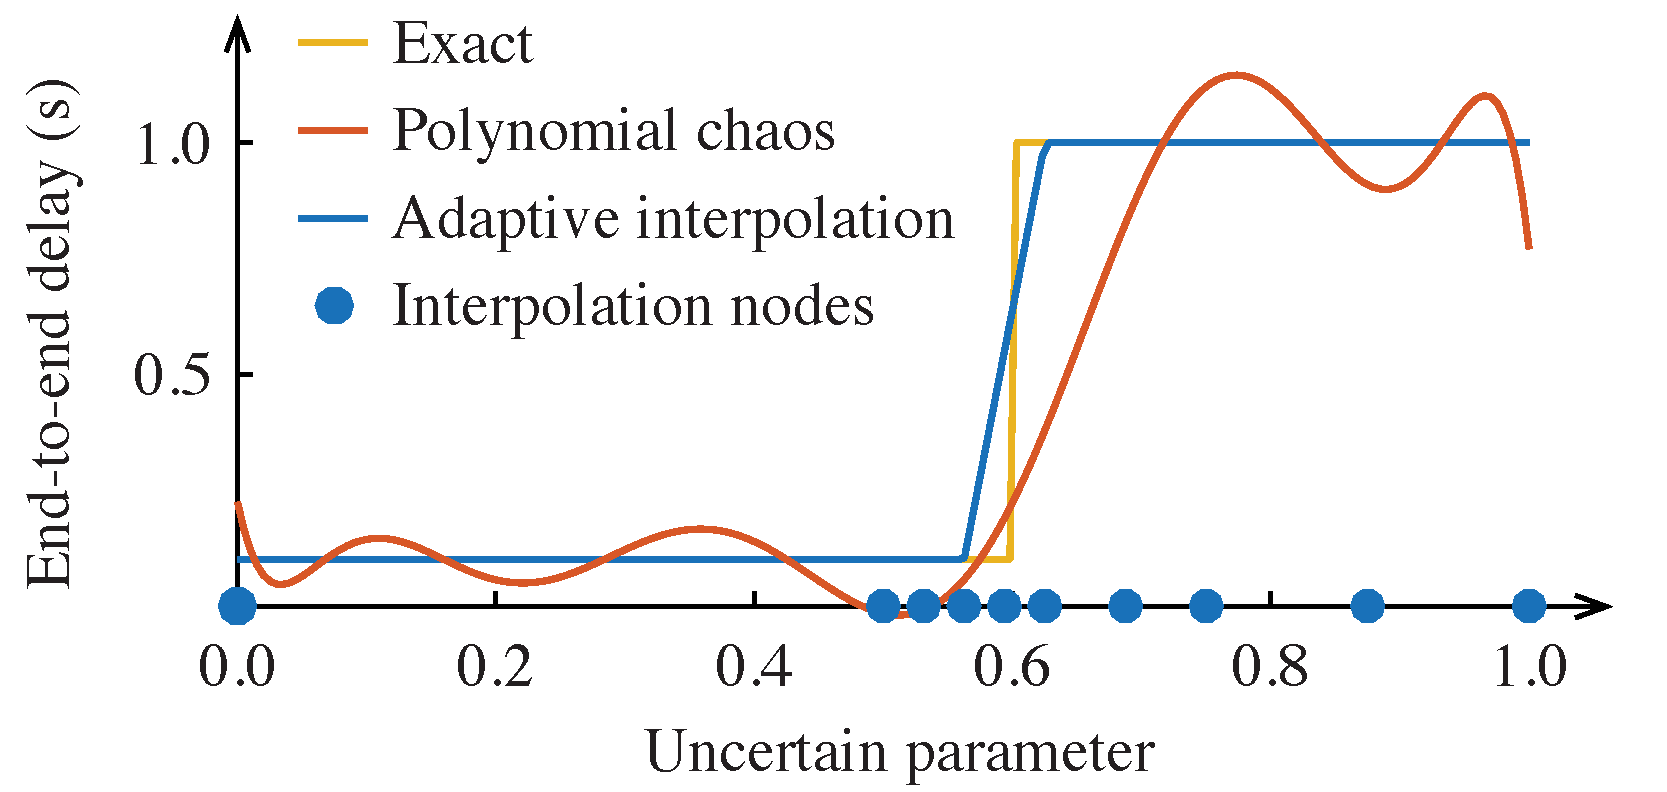
\includegraphics[width=1.0\columnwidth]{include/assets/figures/motivation.pdf}
  \caption{
    An illustration of the accuracy of polynomial chaos expansions and adaptive
    interpolation applied to a non-smooth quantity of interest.
  }
\flab{motivation} \end{figure}

The ability to tackle non-smooth problems is important for the designer of
multiprocess systems. It is especially urgent in the context of digital sources
of uncertainty since the variability due to such sources often lacks smoothness
and might even have discontinuities. Analog sources of uncertainty are forgiving
in this regards due to their physical nature, and polynomial-based
approximations generally work well for them, as in \cite{bhardwaj2008, lee2013,
ukhov2014, ukhov2015}. In order to explore the above concern better, let us
consider a toy example. Suppose that our ``multiprocessor'' system has only one
processing element, and it is running an application with only one task. Suppose
further that the task has two branches and takes either of them depending on the
input data. Assume that one branch takes 0.1~s to execute and has probability
0.6, and the other branch takes 1~s and has probability 0.4. Our goal is to find
the distribution of the end-to-end delay of the application. In this example,
the end-to-end delay coincides with the execution time of the task; hence, we
already know the answer. Let us pretend that we do not and try to apply several
techniques in order to find it.

Suppose the above scenario is modeled by a random variable $\u$ uniformly
distributed in $[0, 1]$: the execution time of the task is 0.1~s if $\u \in [0,
0.6]$, and it is 1~s if $\u \in (0.6, 1]$. The response in this case is a step
function, which is illustrated by the yellow line in \fref{motivation}. First,
we try to approximate the end-to-end delay by constructing a \abbr{PC} expansion
founded on the Legendre polynomial basis \cite{xiu2010}. The orange line in
\fref{motivation} shows a ninth-order \abbr{PC} expansion, which uses 10 points.
It can be seen that the approximation is poor, not to mention negative
end-to-end delays. The observed oscillating behavior is the well-known Gibbs
phenomenon, stemming from the steepness of the response. Now we let our
framework make use of the same number of points as the \abbr{PC} expansion did.
The result is the blue curve in \fref{motivation}, and the adaptively chosen
points are plotted on the horizontal axis. It can be seen that the approximation
is good, and, in fact, it would be indistinguishable from the true response with
a few additional points. One can also note that the adaptive procedure started
to concentrate points at the jump and left the insipid regions on both sides of
the jump with no particular attention. Having constructed such an accurate
representation, one can proceed to the calculation of the probability
distribution of the quantity of interest, which, in general, is done via
sampling followed by such techniques as kernel density estimation. The crucial
point to note here is that this follow-up sampling does not involve the analyzed
multiprocessor system itself and, thus, costs nothing.

The remainder of the paper is organized as follows. Section~\ref{sec:prior-work}
provides an overview of the prior work. In \sref{present-work}, we summarize the
contribution of the present paper. Preliminaries are given in
\sref{preliminaries}. The problem that we address is formulated in
\sref{problem-formulation}, and our solution to the problem is outlined in
\sref{solution}. The proposed framework is presented in \sref{modeling},
\sref{interpolation}, and \sref{analysis}. The experimental results are reported
and discussed in \sref{experimental-results}. Section \ref{sec:conclusion}
concludes the paper.


  \section{Prior Work} \slab{prior-work}
  The techniques developed for probabilistic analysis of multiprocessor systems
are diverse as the area itself and can be classified in many ways. Two natural
classifications originate from the inputs and outputs of the systems that the
techniques have been tailored for. An input, in this context, refers to a source
of uncertainty, and an output refers to a quantity of interest. A technique
tries to give a probabilistic characterization of the latter while taking into
account the effect of the former. The solution that the technique proposes to
solve the problem gives birth to another classification. A solution can be
powered by, for instance, a mathematical framework, statistical method, or
computational algorithm. Let us give an overview of some of the available
techniques from the perspective of the aforementioned classifications.

One of the concerns of an electronic system's designer is process variation
\cite{srivastava2005}. The work in \cite{juan2012} models static steady-state
temperature and accounts for process variation by leveraging the linearity of
Gaussian distributions and time-invariant systems. A stochastic collocation
approach \cite{xiu2010} to static steady-state temperature analysis powered by
Newton polynomials is given in \cite{lee2013}. In \cite{ukhov2014}, transient
temperature analysis is considered, and process variation is address by means of
polynomial-chaos (\abbr{PC}) expansions \cite{xiu2010}. \abbr{PC} expansions
have also been utilized in \cite{ukhov2015} to analyze dynamic steady-state
temperature and parameters of reliability models under process variation.

In order to eliminate or reduce the costs associated with compute experiments in
the context of multiprocessor system design, a number of techniques have been
introduced.

Let us begin with probabilistic timing analysis.

Regarding probabilistic power analysis, the analysis under process variation is
considered in \cite{ukhov2014}.

Let us turn to probabilistic temperature analysis. The analysis under process
variation is considered in \cite{ukhov2014} and \cite{ukhov2015}.


  \section{Our Contribution} \slab{present-work}
  Our work brings the following major contribution: We develop a framework for
probabilistic analysis of electronic systems that is straightforward to use and
is applicable to a wide range of uncertainty-quantification problems.

The usage of the framework is streamlined because it has the same low entrance
requirements as sampling techniques: one only has to be able to evaluate the
quantity of interest given a set of deterministic parameters. Moreover, the
framework can be utilized in scenarios with limited knowledge about the joint
probability distribution of the uncertain parameters, which are common in
practice (to be elaborated on in \sref{parameters}).

The scope of the framework is wide because the framework has a powerful
approximation engine. We make use of adaptive hierarchical interpolation on
sparse grids \cite{jakeman2012, klimke2006, ma2009}, which enable us to tackle
diverse electronic-system-design problems while keeping the associated
computation costs low. In particular, the framework is suitable for nonsmooth
problems, which is an important feature in the context of electronic systems due
to their digital nature, as discussed in \sref{introduction}.

In addition to the aforementioned contribution, we open-source our
implementation \cite{sources}. The implementation is broken down into multiple
standalone libraries, which makes it well disposed to cherry-picked reusage. The
code base also includes the whole experimental setup described in
\sref{experimentation}.


  \section{Preliminaries} \slab{preliminaries}
  Let $\probabilitySpace$ be a probability space where $\outcomes$ is a set of
outcomes, $\sigmaAlgebra \subseteq 2^\outcomes$ is a $\sigma$-algebra, and
$\probabilityMeasure: \sigmaAlgebra \to [0, 1]$ is a probability measure
\cite{durrett2010}. A \rv\ $\h$ defined on $\probabilitySpace$ is an
$\sigmaAlgebra$-measurable function $\h: \outcomes \to \real$. A \rv\ is
uniquely characterized by its (cumulative) distribution function defined by
\begin{equation*}
  \distribution_\h(z) = \probabilityMeasure(\{ \o \in \outcomes: \h(\o) \leq z \}),
\end{equation*}
which is denoted by $\h \sim \distribution_\h$. The expected value and variance
of $\h$ are given by, respectively,
\begin{align}
  & \expectation{\h} = \int_\outcomes \h(\o) \, \d\probabilityMeasure(\o) = \int_\real z \, \d\distribution_\h(z) \hspace{1em} \text{and} \elab{expectation} \\
  & \variance{\h} = \expectation{\h^2} - (\expectation{\h})^2. \elab{variance}
\end{align}

A random vector $\vh = (\h_i)_{i = 1}^n$ is a vector whose elements are \rvs. A
random vector is fully characterized by its distribution function
$\distribution_{\vh}$, denoted $\vh \sim \distribution_{\vh}$. This function is
referred to as a joint or multivariate distribution function, emphasizing the
fact that the variables work together.

An $n$-variate distribution can be expressed as a set of $n$ marginal
(univariate) distributions and an $n$-dimensional copula \cite{nelsen2006}. The
copula is a uniform distribution function on $[0, 1]^n$ (referred to as the
$n$-dimensional unit hypercube) that captures the dependencies between the $n$
individual variables.


  \section{Problem Formulation} \slab{problem-formulation}
  Consider a multiprocessor system composed of two major components: a platform
and an application. The platform consists of a set of heterogeneous processing
elements $\procs = \{ 1, \dots, \np \}$ and is equipped with a thermal package.
The application is given as a set of tasks $\tasks = \{ 1, \dots, \nt \}$. In
what follows, the system will be denoted by $(\procs, \tasks)$.

The designer is assumed to be interested in studying a quantity $\g$ that
characterizes the system described above. The examples include the end-to-end
delay, average power, total energy, maximal temperature, and power and
temperature profiles (data matrices representing discrete snapshots of the
system's dynamics). The quantity $\g$, referred to as the quantity of interest,
depends on a set of parameters that are uncertain at the design stage. In this
work, we focus on those parameters that affect the timing characteristics of the
system such as the execution times of the tasks. The uncertain parameters are
modeled as a random vector $\vu = (\u_i)_{i = 1}^\nu$ with distribution
$\distribution_\vu$. It is important to note that the dependency of $\g$ on
$\vu$, written as $\g(\vu)$, inevitably implies that $\g$ is random for the
designer; however, for a given $\vu$, $\g$ is assumed to be purely
deterministic. Then, the characterization of $\g$ refers to the estimation of
the probability distribution of $\g$, which implicitly delivers all other
quantities such as probabilities, expectations, and variances.

Lastly, for a given $\vu$, the evaluation of $\g$ is assumed to be doable but
expensive (computationally or otherwise). If it was cheap, one could collect
thousands of independent samples of $\g$ and compute all the needed statistics
about $\g$ without involving any framework like the one presented in this paper.

We pursue the following major objectives:
\begin{itemize}

\item \textbf{Objective~1.} Develop a framework for probabilistic analysis of
  the quantity of interest $\g$ characterizing the system $(\procs, \tasks)$
  such that the uncertainty originating from the parameters $\vu$ is taken into
  consideration.

\end{itemize}


  \section{Solution} \slab{solution}
  As noted earlier, making use of an adequate sampling method is a compelling
approach to uncertainty quantification. We would readily apply such a method to
study our quantity of interest $\g$ if only $\g$ had a negligible cost, which it
does not.

Our solution to the above quandary is to construct a light representation of the
heavy $\g$ and study this representation instead of $\g$. The surrogate that we
build is based on adaptive interpolation: $\g$ is evaluated at a number of
strategically chosen collocation nodes, and any other values of $\g$ are
reconstructed on demand (without involving $\g$) using a set of basis functions
mediating between the collected values of $\g$. The benefit of this approach is
in the number of invocations of the quantity of interest $\g$: only a few
evaluations of $\g$ are needed, and the rest of our probabilistic analysis is
powered by the interpolant, which, in contrast to $\g$, has a negligible cost.

Let us delineate the steps involved in the solution process. Recall that $\g$ is
parameterized by the uncertain parameters $\vu$, and these variables are the
only source of randomness. First, we reparameterize $\g$ in terms of an
auxiliary random vector $\vz$ extracted from $\vu$; the necessity of this stage
will become clear later on. Second, we construct an interpolant of $\g$ by
considering $\g$ as a deterministic function of $\vz$ and evaluating $\g$ at a
small set of carefully chosen points. Finally, we estimate the probability
distribution of $\g$ by applying an arbitrary sampling method to the constructed
interpolant of $\g$.

Interpolation of multivariate functions is a challenging task, which should be
approached with a great care. This aspect will be discussed in detail in
\sref{interpolation}. However, before we proceed to interpolation, we first need
to elaborate on the modeling of uncertain parameters and quantities of interest.


  \section{Modeling} \slab{modeling}
  The agenda for this section is as follows. In \sref{parameters}, the uncertain
parameters $\vu$ are transformed into a form suitable for the subsequent
calculations. \updated{This stage is an essential part of our framework, and it
is denoted by $\transformation$ in \fref{example}.} The rest of the subsections,
\sref{time}--\ref{sec:temperature}, serve a strictly illustrative purpose.
\updated{They exemplify the leftmost box in \fref{example} in order to give the
reader a better intuition about the utility of the framework. The subsections
introduce a number of models and a number of metrics $\g$; however, it should be
well understood that the essence of $\g$ is problem specific. In practice, $\g$
stands for an adequate simulator of the system under consideration. The modeling
capabilities of this simulator are naturally inherited by the proposed
framework.}

\subsection{Uncertainty Parameters} \slab{parameters}
The foremost step of our framework is to change the parameterization of the
problem from the random vector $\vu = (\u_i)_{i = 1}^\nu \sim \distribution_\vu$
to an auxiliary random vector $\vz = (\z_i)_{i = 1}^\nz \sim \distribution_\vz$
such that: 1) the support of $\distribution_\vz$ is the unit hypercube $[0,
1]^\nz$, and 2) $\nz \leq \nu$ has the smallest value needed to retain the
desired level of accuracy. The first is standardization, which is done primarily
for convenience. The second is model-order reduction, which identifies and
eliminates excessive complexity and, hence, speeds up the solution process. The
reduction is possible whenever there are dependencies between $(\u_i)_{i =
1}^\nu$, in which case one can find such $(\z_i)_{i = 1}^\nz$, $\nz < \nu$, that
each $\u_i$ can be recovered from $(\z_i)_{i = 1}^\nz$. We shall denote the
overall transformation by $\vu = \transformation(\vz)$ where
\begin{equation} \elab{transformation}
  \transformation: \real^\nu \to [0, 1]^\nz.
\end{equation}
For any point $\vz \in [0, 1]^\nz$, we are now able to compute the corresponding
$\vu$ and, consequently, the quantity of interest $\g$ as $(\g \circ
\transformation)(\vz) = \g(\transformation(\vz)) = \g(\vu)$; recall also
\sref{problem}.

Let us consider an example of $\transformation$ in order to understand the
concept better. To this end, we begin by assuming that the distribution of $\vu
= (\u_i)_{i = 1}^\nu$, $\distribution_\vu$, is given as a set of marginal
distribution functions $\{ \distribution_{\u_i} \}_{i = 1}^\nu$ and a copula
\cite{nelsen2006} (see also \sref{preliminaries}). Furthermore, the copula is
assumed to be a Gaussian copula whose correlation matrix is $\correlation \in
\real^{\nu \times \nu}$.

It is important to note the following. A set of marginals and a copula entirely
characterize the joint distribution of $\vu$, that is, $\distribution_\vu$.
However, we consider this distribution as an approximation rather than as the
true one. The knowledge of the true joint would be an impractical assumption to
make. A more realistic assumption is the availability of the marginals and
correlation matrix of $\vu$. In general, these two pieces are not sufficient to
recover the joint of $\vu$; however, the joint can be approximated well by
accompanying the available marginals by a Gaussian copula constructed based on
the available correlation matrix; see \cite{liu1986} and also \cite{ukhov2014}.
Hence, a set of marginals and a Gaussian copula are practical inputs to
probabilistic analysis.

The number of variables, which is so far $\nu$, has a significant impact on the
complexity of the problem at hand. Therefore, an important component of our
framework is model-order reduction, which we shall base on the discrete
Karhunen--Lo\`{e}ve decomposition, also known as the principal component
analysis. We proceed as follows. Since any correlation matrix is real and
symmetric, $\correlation$ admits the eigendecomposition: $\correlation = \m{V}
\m{\Lambda} \m{V}^T$ where $\m{V} \in \real^{\nu \times \nu}$ is an orthogonal
matrix whose columns are the eigenvectors of $\correlation$, and $\m{\Lambda} =
\diag(\lambda_i)_{i = 1}^\nu$ is a diagonal matrix whose diagonal elements are
the eigenvalues of $\correlation$. The eigenvalues $(\lambda_i)_{i = 1}^\nu$
correspond to the variances of the corresponding components revealed by the
decomposition. The model-order reduction boils down to selecting those major
components whose cumulative contributions to the total variance is above a
certain threshold. Formally, assuming that $(\lambda_i)_{i = 1}^\nu$ are sorted
in the descending order and given a threshold $\eta \in (0, 1]$ specifying the
fraction of the total variance to be preserved, we identify the smallest $\nz$
such that
\begin{equation} \elab{reduction}
  \frac{\sum_{i = 1}^\nz \lambda_i}{\sum_{i = 1}^\nu \lambda_i} \geq \eta.
\end{equation}
Denote by $\tilde{\m{V}} \in \real^{\nu \times \nz}$ and $\tilde{\m{\Lambda}}
\in\real^{\nz \times \nz}$ the matrices obtained by truncating $\m{V}$ and
$\m{\Lambda}$, respectively, to preserve only the first $\nz$ components where
$\nz$ is as shown above.

Now, the transformation $\transformation$ in \eref{transformation} is
\begin{equation} \elab{transformation-concrete}
  \vu = \distribution_\vu^{-1} \left( \Phi\left( \tilde{\m{V}} \tilde{\m{\Lambda}}^\frac{1}{2} \, \Phi^{-1}(\vz) \right) \right)
\end{equation}
where the \rvs\ $\vz = (\z_i)_{i = 1}^\nz$ are independent and uniformly
distributed on $[0, 1]^\nz$; $\Phi$ and $\Phi^{-1}$ are the distribution
function of the standard Gaussian distribution and its inverse, respectively,
which are applied elementwise; and $\distribution_\vu^{-1} =
\distribution_{\u_1}^{-1} \times \cdots \times \distribution_{\u_\nz}^{-1}$ is
the Cartesian product of the inverse marginal distributions of $\vu$, which are
applied to the corresponding element of the vector yielded by $\Phi$. In the
absence of correlations, \eref{transformation-concrete} is simply $\vu =
\distribution_\vu^{-1}(\vz)$, and no model-order reduction is possible ($\nu =
\nz$). It might be interesting to note that, using the above transformation, the
distribution $\vu$ gets ``baked'' in $\g$ because it ``disappears'' when $\g$ is
viewed as a function of $\vz$, distributed uniformly.

To summarize, we have found such a transformation $\transformation$ and the
corresponding random vector $\vz \sim \distribution_\vz$ that: 1)
$\distribution_\vz$ is supported by $[0, 1]^\nz$, and 2) $\vz$ has the smallest
number of dimensions $\nz$ needed to preserve $\eta$ portion of the variance.


\subsection{Application Timing} \slab{time}
Suppose the application is given as a directed acyclic graph. The vertices
represent tasks, and the edges data dependency between these tasks. Suppose
further that a static cyclic scheduling policy is utilized. Note, however, these
assumptions are orthogonal to our framework: the framework can be applied to any
application model and any scheduling policy.

Each task has a start and a finish time. For task $i$, denote these two time
moments by $\b_i$ and $\d_i$, respectively, and let $\vb = (\b_i)_{i=1}^\nt$ and
$\vd = (\d_i)_{i=1}^\nt$. Other timing characteristics of the application can be
derived from $(\vb, \vd)$. An example is the end-to-end delay, which is the
difference between the finish time of the latest task and the start time of the
earliest task:
\begin{equation} \elab{end-to-end-delay}
  \text{End-to-end delay} = \max_{i = 1}^\nt \, \d_i - \min_{i = 1}^\nt \, \b_i.
\end{equation}

Suppose the execution times of the tasks depend on $\vu$ (see \sref{problem}).
Then the tuple $(\vb, \vd)$ depends on $\vu$. \updated{Then the end-to-end delay
given in \eref{end-to-end-delay} depends on $\vu$ and constitutes a potential
metric $\g$.} Note that this $\g$ is nondifferentiable as the $\max$ and $\min$
functions are such. Hence, $\g$ is nonsmooth, which renders \up{PC} expansions
and similar techniques inadequate for this problem, as illustrated in
\sref{introduction}.

\begin{remark} \rlab{smoothness}
In general, the behavior of $\g$ with respect to continuity, differentiability,
and smoothness cannot be inferred from the behavior of $\vu$. Even when the
parameters are perfectly behaved, $\g$ can still and likely will exhibit
nondifferentiability or even discontinuity, which depends on how $\g$ works
internally. For example, as shown in \cite{tanasa2015}, even if execution times
of tasks are continuous, due to the actual scheduling policy, end-to-end delays
are very often discontinuous.
\end{remark}


\subsection{Power Consumption} \slab{power}
Denote the number of processing elements present on the platform by $\np$. Let
the dynamic power consumed by task $j$ when running on processing element $i$ be
fixed during the execution of the task and denote this dynamic power by
$\p^\dynamic_{ij}$. The fact that $\p^\dynamic_{ij}$ is constant might seem
restrictive. However, one should keep in mind that it is a example. Our
framework does not have such a restriction. Even in this simple model, the
modeling accuracy can be substantially improved by representing large tasks as
sequences of smaller tasks.

Let the vector $\vp(\t) = (\p_i(\t))_{i = 1}^{\np}$ capture the total power
consumption of the system at time $\t$. This vector is related to the dynamic
power introduced above as follows:
\begin{equation} \elab{power}
  \p_i(\t) = \sum_{j = 1}^\nt \p^\dynamic_{ij} \: \delta_{ij} (\t) + \p^\static_i(\t), \hspace{1em} \text{for $i = 1, \dots, \np$},
\end{equation}
where $\delta_{ij}(\t)$ is an indicator function (outputs either zero or one) of
the event that processing element $i$ executes task $j$ at time $\t$, and
$\p^\static_i(\t)$ is the static power consumed by processing element $j$ at
time $\t$. The last component depends on time because the leakage power and
temperature are interdependent \cite{liu2007}, and temperature changes over time
(see the next subsection).

Given a set of $\ns$ points on the timeline $\{ \t_i \}_{i = 1}^\ns$,
\eref{power} can be used to construct a power profile of the system as follows:
\[
  \mP = (\p_i(\t_j))_{i = 1, j = 1}^{\np, \ns} \in \real^{\np \times \ns}.
\]
The above is essentially a matrix where row $i$ captures the power consumed by
processing element $i$ at the $\ns$ time moments.

The total energy consumed by the system during an application run can be
computed by integrating \eref{power} over the time span of the
application---which is demarcated by the minuend and subtrahend in
\eref{end-to-end-delay}---and the corresponding integral can be estimated using
the power profile as follows:
\begin{equation} \elab{total-energy}
  \text{Total energy} = \sum_{i = 1}^\np \int \p_i(\t) \, \d\t \approx \sum_{i = 1}^\np \sum_{j = 1}^\ns \p_i(\t_j) \, \Delta\t_j
\end{equation}
where $\Delta\t_j$ is either $\t_j - \t_{j - 1}$ or $\t_{j + 1} - \t_j$,
depending on how power values are encoded in $\mP$. The assumption that
\eref{total-energy} is based on is that each $\Delta\t_i$ is sufficiently small
so that the power consumed within the interval does not change significantly.

Since the tuple $(\vb, \vd)$ depends on $\vu$, the power consumption of the
system depends on $\vu$ too. Consequently, the total energy given in
\eref{total-energy} depends on $\vu$ and is a candidate for $\g$.


\subsection{Heat Dissipation} \slab{temperature}
Based on the specification of the platform including its thermal package, an
equivalent thermal \up{RC} circuit is constructed \cite{skadron2004}. The
circuit comprises $\nn$ thermal nodes, and its structure depends on the intended
level of granularity, which impacts the resulting accuracy. For clarity, we
assume that each processing element is mapped onto one corresponding node, and
the thermal package is represented as a set of additional nodes. As before, let
us remind that the \up{RC} model is an example; other models can be used with
our framework equally well.

The thermal dynamics of the system are modeled using the following system of
differential-algebraic equations \cite{ukhov2014, ukhov2012}:
\begin{subnumcases}{\elab{thermal-system}}
  \mC \frac{\d\vs(\t)}{\d\t} + \mG \vs(\t) = \mM \vp(\t) \\
  \vq(\t) = \mM^T \vs(\t) + \vq_\ambient
\end{subnumcases}
The coefficients $\mC \in \real^{\nn \times \nn}$ and $\mG \in \real^{\nn \times
\nn}$ are a diagonal matrix of thermal capacitance and a symmetric,
positive-definite matrix of thermal conductance, respectively. The vectors
$\vp(\t) \in \real^\np$,  $\vq(\t) \in \real^\np$, and $\vs(\t) \in \real^\nn$
correspond the system's power, temperature, and internal state at time $\t$,
respectively. The vector $\vq_\ambient \in \real^\np$ contains the ambient
temperature. The matrix $\mM \in \real^{\nn \times \np}$ is a mapping that
distributes the power consumption of the processing elements across the thermal
nodes; without loss of generality, $\mM$ is a rectangular diagonal matrix whose
diagonal elements are equal to one.

Given a set of $\ns$ points on the timeline $\{ \t_i \}_{i = 1}^\ns$,
\eref{thermal-system} can be used to compute a temperature profile of the system
as follows:
\begin{equation*}
  \mQ = (\q_i(\t_j))_{i = 1, j = 1}^{\np, \ns} \in \real^{\np \times \ns}.
\end{equation*}
Then the maximum temperature of the system can be estimated using the
temperature profile as follows:
\begin{equation} \elab{maximum-temperature}
  \text{Max temperature} = \max_{i = 1}^\np \, \sup_{\t} \, \q_i(\t) \approx \max_{i = 1}^\np \max_{j = 1}^\ns \, \q_i(\t_j).
\end{equation}

Since the power consumption of the system is affected by $\vu$ (see
\sref{power}), the system's temperature is affected by $\vu$ as well. Therefore,
the temperature in \eref{maximum-temperature} can be considered as a quantity of
interest $\g$. Note that, due to the maximization involved, the quantity is
nondifferentiable and, hence, cannot be adequately addressed using polynomial
approximations, specially taking into account the concern in \rref{smoothness}.


To sum up, we have discussed the transformation that needs to be applied to
$\vu$ prior to the interpolation of $\g$. \updated{We have also covered three
aspects of electronic systems, namely, timing, power, and temperature, and
introduced a number of metrics associated with them; we shall come back to these
metrics in the section on experimental results, \sref{experimentation}.}


  \section{Interpolation} \slab{interpolation}
  In this section, we present the interpolation algorithm that forms the core of
the proposed framework for probabilistic analysis of electronic systems. The
algorithm is based on the work in \cite{jakeman2012, klimke2006, ma2009}, and it
features a sparse-grid structure, hierarchical construction, and hybrid
adaptivity. The benefits of these features are interconnected and can be
summarized as follows: the ability to mitigate the curse of dimensionality and,
thereby, tackle multidimensional problems; the ability to perform gradual
refinement of the approximation with a natural error control; and the ability to
make the refinement fine-grained and, hence, gain further efficiency.

Let $\f$ be a function that we would like to approximate. The function is
assumed to be in $\continuous([0, 1]^\nin)$, the space of continuous functions
in the unit hypercube $[0, 1]^\nin$. The assumption is a formality, and the
interpolation algorithm discussed in \sref{implementation} can be applied to
functions with finite discontinuities as well, which is actually the case in the
example given in \fref{motivation}. Furthermore, the domain $[0, 1]^\nin$ is
merely standardization rather than a restriction.

In what follows, we shall gradually construct an efficient interpolant for $\f$.
Efficiency here refers to the number of collocation nodes required to achieve a
certain accuracy level.

\subsection{Tensor Product} \slab{tensor-product}
In one dimension ($\nin = 1$), $\f$ is approximated by virtue of the following
interpolation formula:
\begin{equation} \elab{tensor-1d}
  \tensor{i}(\f) := \sum_{j \in \index_i} \f(\x_{ij}) \, \e_{ij}.
\end{equation}
The superscript $i \in \natural$ signifies the level of interpolation; $\X_i =
\{ \x_{ij} \}_{j \in \index_i} \subset [0, 1]$ are the collocation nodes; $\E_i
= \{ \e_{ij} \}_{j \in \index_i} \subset \continuous([0, 1])$ are the basis
functions; and $\index_i = \{ j - 1 \}_{j = 1}^{n_i}$ is an index set
enumerating (starting from zero) the nodes and functions that belong to level
$i$. We shall refer to the subscript $j \in \index_i$ as the order of a node or
function. The choice of the collocation nodes and basis functions is an
important concern, and it will be discussed thoroughly later on.

In multiple dimensions ($\nin > 1$), $\f$ is approximated by the tensor product
of $\nin$ one-dimensional interpolants:
\begin{equation} \elab{tensor}
  \tensor{\vi}(\f) := \left( \bigotimes_{k = 1}^\nin \tensor{i_k} \right)(\f) = \sum_{\vj \in \index_\vi} \f(\vx_{\vi\vj}) \, \e_{\vi\vj}
\end{equation}
where $\vi = (i_k)_{k = 1}^\nin \in \natural^\nin$ and $\vj = (j_k)_{k = 1}^\nin
\in \natural^\nin$ are multi-indices specifying levels and orders, respectively,
for each of the dimensions, and $\index_\vi := \index_{i_1} \times \cdots \times
\index_{i_\nin}$ is a multi-index set obtained by computing the tensor product
of one-dimensional index sets. In the above formula,
\begin{align}
  \X_\vi &= \X_{i_1} \times \cdots \times \X_{i_\nin} \elab{collocation-nodes} \\
         &= \left\{ \vx_{\vi\vj} = (\x_{i_k j_k})_{k = 1}^\nin \right\}_{\vj \in \index_\vi} \subset [0, 1]^\nin \nonumber
\end{align}
and
\begin{equation} \elab{basis-functions}
  \E_\vi = \bigotimes_{k = 1}^\nin \E_{i_k}
         = \left\{ \e_{\vi\vj} = \bigotimes_{k = 1}^\nin \e_{i_k j_k} \right\}_{\vj \in \index_\vi} \subset \continuous([0, 1]^\nin)
\end{equation}
are the collocation nodes and basis functions, respectively, corresponding to
multi-index $\vi$. In \eref{basis-functions}, for any $\vx \in [0, 1]^\nin$,
\begin{equation} \elab{basis-function}
  \e_{\vi\vj}(\vx) = \left( \bigotimes_{k = 1}^\nin \e_{i_k j_k} \right)(\vx) := \prod_{k = 1}^\nin \e_{i_k j_k}(\x_k).
\end{equation}
Lastly, the cardinality of $\index_\vi$ is as follows:
\begin{equation} \elab{tensor-cardinality}
  \n_\vi = \prod_{k = 1}^\nin \n_{i_k}.
\end{equation}
Equation \eref{tensor-cardinality} elucidates the prohibited expense of the
tensor-product construction shown in \eref{tensor} for multidimensional
problems: the number of nodes grows exponentially as $\nin$ increases. However,
\eref{tensor} serves well as a building block for more efficient algorithms,
which we discuss next.

\begin{remark}
Each dimension can have its own rule defining the distribution of collocation
node with respect to each level. Similarly, the basis functions of one dimension
can differ from the basis functions of another. For simplicity and clarity of
presentation, this aspect is not covered in this paper.
\end{remark}


\subsection{Smolyak Algorithm} \slab{smolyak-algorithm}
One of the central algorithms in the field of high-dimensional integration and
interpolation is the Smolyak algorithm \cite{smolyak1963}. The technique was
developed in the 1960s by Sergey Smolyak, and its impact is comparable to the
one of Monte Carlo sampling. Intuitively speaking, the algorithm takes a number
of small tensor-product structures and composes them in such a way that the
resulting grid has a drastically reduced number of nodes while preserving the
approximating power of the full tensor-product construction for the classes of
functions that one is typically interested in integrating or interpolating
\cite{klimke2006}.

The Smolyak interpolant for $\f$ is as follows:
\begin{equation} \elab{smolyak}
  \smolyak{l}(\f) := \sum_{l - \nin + 1 \leq |\vi|_1 \leq l} (-1)^{l - |\vi|_1} \, {\nin - 1 \choose l - |\vi|_1} \, \tensor{\vi}(\f)
\end{equation}
where $l \in \natural$ is the level of Smolyak's interpolation, and $|\vi|_1 :=
i_1 + \dots + i_\nin$. We see that the algorithm is indeed just a peculiar
composition of cherry-picked tensor products. However, the formula has an
implication of paramount importance: the quantity of interest needs to be
evaluated only at the nodes of the sparse grid underpinning \eref{smolyak}:
\begin{equation} \elab{smolyak-grid}
  \Y^l = \bigcup_{l - \nin + 1 \leq |\vi|_1 \leq l} \X^\vi.
\end{equation}
The cardinality of the above set does not have a general closed-form formula;
however, it can be several orders of magnitude smaller than the one of the full
tensor product given in \eref{tensor-cardinality}, which depends on the
dimensionality of the problem at hand and the one-dimensional rules utilized.

A better intuition about the properties of Smolyak's construction can be
obtained by rewriting \eref{smolyak} in an incremental form. To this end, let
$\Delta\tensor{-1}(\f) := 0$,
\begin{align}
  & \Delta\tensor{i}(\f) := (\tensor{i} - \tensor{i - 1})(\f), \text{ and} \elab{tensor-delta-1d} \\
  & \Delta\tensor{\vi}(\f) := (\Delta\tensor{i_1} \otimes \cdots \otimes
  \Delta\tensor{i_\nin})(\f). \nonumber
\end{align}
Then, \eref{smolyak} is identical to
\begin{equation} \elab{smolyak-incremental}
  \smolyak{l}(\f) = \sum_{|\vi|_1 \leq l} \Delta\tensor{\vi}(\f) = \smolyak{l - 1}(\f) + \sum_{|\vi|_1 = l} \Delta\tensor{\vi}(\f)
\end{equation}
where $\smolyak{-1}(\f) := 0$. It can be seen that a Smolyak interpolant can be
refined efficiently: the work done to attain one accuracy level can be entirely
recycled to go one level up.

The sparsity and incremental refinement of Smolyak's approach, which are shown
in \eref{smolyak-grid} and \eref{smolyak-incremental}, respectively, are
remarkable properties \perse, but they can be taken even further. To this end,
let $\Delta\X^{-1} := \emptyset$,
\begin{align*}
  & \Delta\X^i := \X^i \setminus \X^{i - 1}, \text{ and} \\
  & \Delta\X^\vi := \Delta\X^{i_1} \times \cdots \times \Delta\X^{i_\nin}.
\end{align*}
Then, \eref{smolyak-grid} can be rewritten as
\begin{equation} \elab{smolyak-grid-incremental}
  \Y^l = \bigcup_{|\vi|_1 \leq l} \Delta\X^\vi = \Y^{l - 1} \cup \bigcup_{|\vi|_1 = l} \Delta\X^\vi,
\end{equation}
which is analogous to \eref{smolyak-incremental}. It can be seen now that it is
beneficial for refinement to have $\X^{i - 1}$ be entirely included in $\X^i$
since, in that case, the cardinality of $\Y^l \setminus \Y^{l - 1} =
\bigcup_{|\vi|_1 = l} \Delta\X^\vi$ derived from \eref{smolyak-grid-incremental}
decreases. In words, the values of $\f$ obtained on lower levels can be reused
to attain higher levels if the grid grows without abandoning its previous
structure. With this in mind, the rule used for generating successive sets of
points $\{ \X^i \}_{i \in \natural}$ should be chosen to be nested, that is, in
such a way that $\X^i$ contains all nodes of $\X^{i - 1}$. By doing so, the
incremental refinement really starts to shine.

Lastly, we need to impose one additional property in order to rewrite
\eref{smolyak-incremental} in a hierarchical form. Namely, we require the
interpolants of higher levels to represent exactly the interpolants of lower
levels. In one dimension, it means that
\begin{equation} \elab{tensor-exactness}
  \tensor{i - 1}(\f) = \tensor{i}(\tensor{i - 1}(\f)).
\end{equation}
The condition in \eref{tensor-exactness} can be satisfied by an appropriate
choice of collocation nodes and basis functions, which will be discussed later.
If \eref{tensor-exactness} holds, using \eref{tensor-1d} and
\eref{tensor-delta-1d},
\[
  \Delta\tensor{i}(\f) = \sum_{j \in \Delta\index(i)} \left( \f(\x^i_j) - \tensor{i - 1}(\f)(\x^i_j) \right) \, \e^i_j
\]
where $\Delta\index(i) := \{ j \in \index(i): \x^i_j \in \Delta\X^i \}$. The
above sum is over $\Delta\X^i$ due to the fact that the difference in the
parentheses is zero whenever $\x^i_j \in \X^{i - 1}$ since $\X^{i - 1} \subset
\X^i$. In multiple dimensions, using the Smolyak formula, we have
\begin{equation} \elab{tensor-delta}
  \Delta\tensor{\vi}(\f) = \sum_{\vj \in \Delta\index(\vi)} \left( \f(\vx^\vi_\vj) - \smolyak{|\vi|_1 - 1}(\f)(\vx^\vi_\vj) \right) \, \e^\vi_\vj
\end{equation}
where $\Delta\index(\vi) := \{ \vj \in \index(\vi): \vx^\vi_\vj \in \Delta\X^\vi
\}$. The delta
\begin{equation} \elab{surplus}
  \surplus(\vx^\vi_\vj) := \f(\vx^\vi_\vj) - \smolyak{|\vi|_1 - 1}(\f)(\vx^\vi_\vj)
\end{equation}
is called a hierarchical surplus. When increasing the interpolation level, this
surplus is nothing but the difference between the actual value of $\f$ at a new
node and the approximation of this value computed by the interpolant constructed
so far.

The final formula for nonadaptive hierarchical interpolation is obtained by
substituting \eref{tensor-delta} into \eref{smolyak-incremental}:
\begin{equation} \elab{smolyak-hierarchical}
  \smolyak{l}(\f) = \smolyak{l-1}(\f) + \sum_{|\vi|_1 = l} \, \sum_{\vj \in \Delta\index(\vi)} \surplus(\vx^\vi_\vj) \, \e^\vi_\vj
\end{equation}
where $\surplus(\vx^\vi_\vj)$ is computed according to \eref{surplus}.


\subsection{Collocation Nodes} \slab{collocation-nodes}
A sparse grid that is fully nested and well suited for local adaptivity, which
we requested previous, can be constructed using the (one-dimensional)
Newton--Cotes rule \cite{klimke2006, ma2009}. For each level, the rule is merely
a set of equidistant nodes on an interval, which is $[0, 1]$ in our case.

\begin{remark}
Equidistant nodes are known to perform poorly when the interpolating functions
are polynomials (Runge's phenomenon). However, it is not a concern for us as our
basis functions are not exposed to this problem.
\end{remark}

The rule comes in two flavors: closed and open. The only difference between the
two is that the former includes the endpoints, that is, 0 and 1, while the
latter does not. Now, at the end of \sref{smolyak-algorithm}, we postulated that
the assumption in \eref{tensor-exactness} was needed to proceed. The closed rule
satisfies this assumption while the open one violates it close to the boundaries
of the interval. However, as noted in \cite{klimke2006}, the open Newton--Cotes
rule is a viable option since it performs well in practice. We were able to
achieve better results using the open rule, and, therefore, we have decided to
present it in the paper.

\begin{figure}[t]
  \centering
  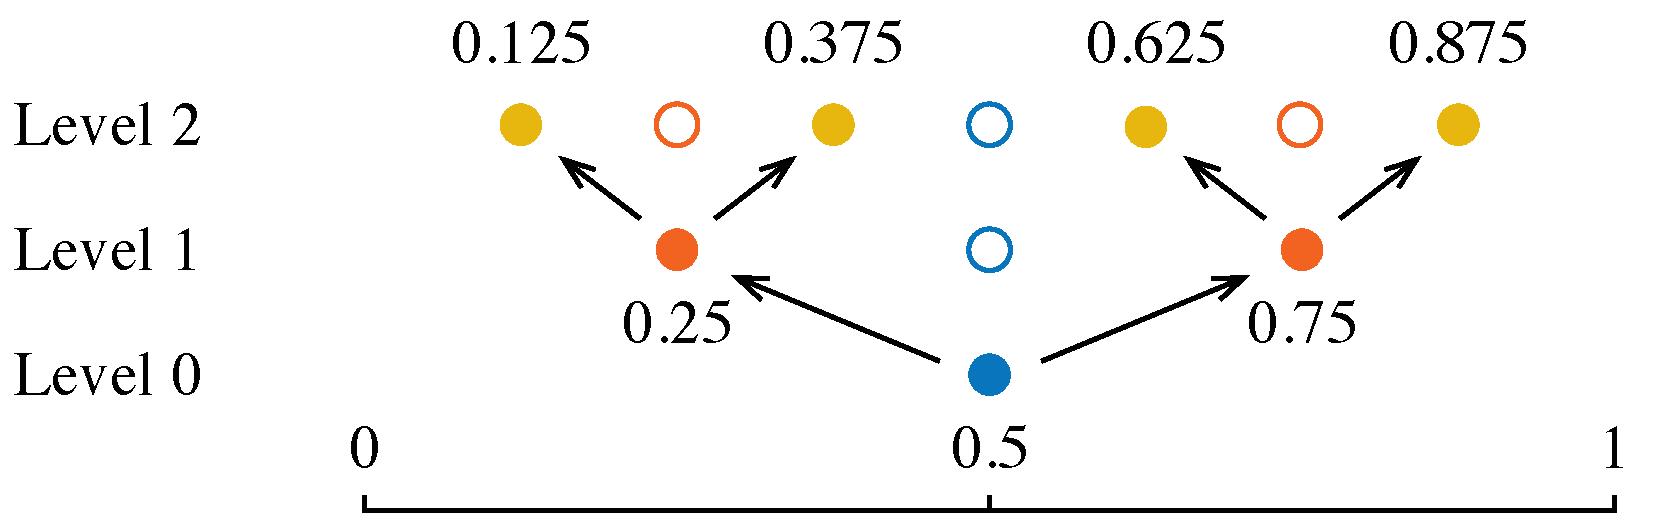
\includegraphics[width=1.0\columnwidth]{include/assets/figures/rule.pdf}
  \caption{
    An illustration of the open Newton--Cotes rule on $[0, 1]$. On each level,
    the dots correspond to the nodes introduced by that particular level, and
    the wholes correspond to the nodes inherited from the previous levels.
  }
  \flab{rule}
\end{figure}

The open Newton--Cotes rule of level $i \in \natural$ is
\begin{equation} \elab{newton-cotes-grid}
  \X_i = \left\{ x_{ij} = \frac{j + 1}{\n_i + 1}: j \in \index_i \right\}
\end{equation}
where $\index_i = \left\{ 0, \dots, \n_i - 1 \right\}$ with $\n_i = 2^{i + 1} -
1$. The first three levels of the rule are depicted in \fref{rule}. It can be
seen that the number of nodes (in one dimension) grows as 1, 3, 7, 15, 31, and
so on, and the rule is fully nested. In multiple dimensions, the nodes are
formed as shown in \eref{collocation-nodes}.

Figure~\ref{fig:rule} also illustrates a refinement procedure suitable for this
grid. The arrows emerging from a node connect the node with its next-level
neighbors. The number of such neighbors is two in one dimension and $2 \nin$ in
general. Formally, for a pair $(\vi, \vj)$, the neighbor pairs are
\[
  \left\{ \Big( (i_1, \dots, i_k + 1, \dots, i_\nin), (j_1, \dots, 2 j_k + c, \dots j_\nin) \Big) \right\}_{k, c}
\]
for $k = 1, \dots, \nin$ and $c \in \{ 0, 2 \}$. Whenever a node is chosen for
refinement, some or all of its neighbors can be added to the interpolant. One
possible strategy is to include all $2 \nin$ neighbors, which is what we shall
do.

\begin{remark}
It is important to note that an arbitrary set of nodes identified by some pairs
$\{ (\vi_k, \vj_k) \}_k$ does not necessarily correspond to a valid
construction. In order to have a valid construction, the multi-indices $\{ \vi_k
\}_k$ should satisfy a so-called admissibility condition \cite{klimke2006}. The
condition is diligently satisfied when the refinement is undertaken level by
level following neighbor connections, which is what we do.
\end{remark}

First of all, looking at \eref{smolyak-hierarchical}, it is not clear what the
interpolation level $\l$ should be in order to achieve a certain accuracy level.
When should we stop?


\subsection{Basis Functions} \slab{basis-functions}
\begin{figure}[t]
  \centering
  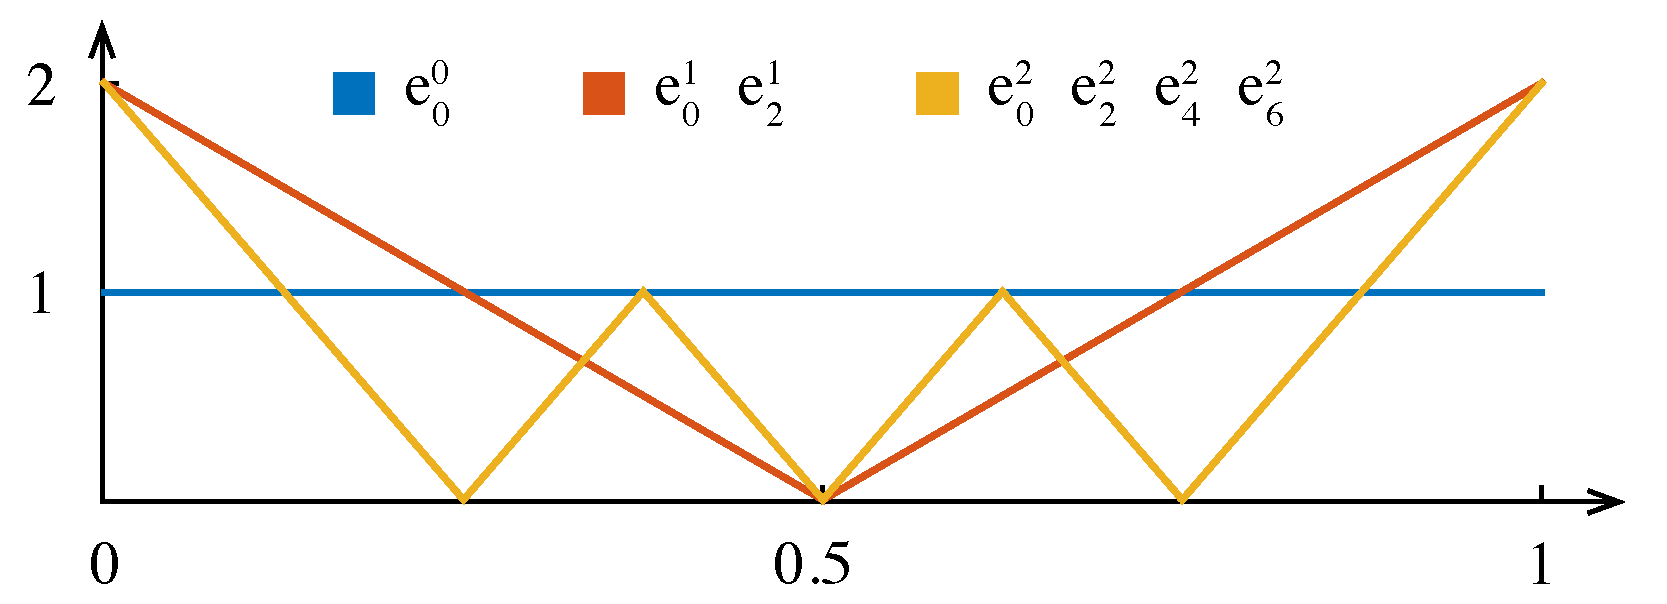
\includegraphics[width=1.0\columnwidth]{include/assets/figures/basis.pdf}
  \vspace{-1.5em}
  \caption{
    The first three levels of the basis described in \sref{basis}.
  }
  \flab{basis}
\end{figure}

The basis functions that go hand in hand with the open Newton--Cotes rule are
the following piecewise linear functions. For $i = 0$ and $j = 0$,
\[
  \e_{00}(\x) = 1.
\]
For $i > 0$ and $j = 0$ (close to the left endpoint),
\[
  \e_{i0}(\x) = \begin{cases}
    2 - \left( \n_i + 1 \right) \x, & \text{if } \x < \frac{2}{\n_i + 1}, \\
    0, & \text{otherwise}.
  \end{cases}
\]
For $i > 0$ and $j = \n_i - 1$ (close to the right endpoint),
\[
  \e_{i(\n_i - 1)}(\x) = \begin{cases}
    \left( \n_i + 1 \right) \x - \n_i + 1, & \text{if } \x > \frac{\n_i - 1}{\n_i + 1}, \\
    0, & \text{otherwise}.
  \end{cases}
\]
In other cases,
\[
  \e_{ij}(\x) = \begin{cases}
    1 - \left( \n_i + 1 \right)|\x - \x_{ij}|, & \text{if } |\x - \x_{ij}| < \frac{1}{\n_i + 1}, \\
    0, & \text{otherwise}.
  \end{cases}
\]
The basis functions corresponding to the first three levels of one-dimensional
interpolation are depicted in \fref{basis}. Note that $\e_{11}$, $\e_{21}$,
$\e_{23}$, and $\e_{25}$ are not depicted as they are not involved in the
hierarchical construction. In multiple dimensions, the basis functions are
formed as shown in \eref{basis-functions}.

Lastly, let us mention the volumes (integrals over the whole domain) of the
basis functions denoted by $\w_{ij}$; they will be needed in the future. Namely,
$\w_{00} = 1$ and, for $i > 0$,
\begin{equation} \elab{volume}
  \w_{ij} := \int_0^1 \e_{ij}(\x) \, \d\x = \begin{cases}
    \frac{2}{\n_i + 1}, & \text{if } j \in \{ 0, \n_i - 1 \}, \\
    \frac{1}{\n_i + 1}, & \text{otherwise}.
  \end{cases}
\end{equation}
In multiple dimensions, the volumes are products of the one-dimensional
components, analogous to \eref{basis-function}.

\begin{remark}
Instead of piecewise linear functions, one can also utilize locally supported
polynomials of higher orders \cite{jakeman2012}. However, we did not observe
much improvement and, therefore, do not discuss this alternative in the paper.
\end{remark}


\subsection{Adaptivity} \slab{adaptivity}
We are ready to discuss adaptivity, and we begin by reiterating briefly out
motivation. Imagine a function that is nearly flat on the first half of $[0, 1]$
and rather irregular on the other. Under these circumstances, it is natural to
expect that, in order to attain the same accuracy, the first half would require
much fewer collocation nodes than the other one; recall the example given in
\fref{motivation}. However, if we followed the construction procedure described
so far, we would not be able to benefit from the peculiar behavior: we would
treat both sides equally and would add all the nodes of each level.

The solution to the above problem is to make the interpolation algorithm
adaptive. First of all, we need to find a way to measure how good our
approximation is at any point in the domain of $\f$. Then, when taking an
interpolation step, instead of bombarding $\f$ with all the nodes that can be
legitimately added to the interpolant at that step, we will only include those
nodes that are located in the regions with poor accuracy as indicated by the
yet-to-be-found accuracy metric. The outlined strategy practically means that
$\Delta\lindex_\l$ and $\Delta\oindex_\vi$ in \eref{smolyak-hierarchical} will
be only subsets of what is possible at step $\l$.

\begin{remark}
It is important to note that, in general, an arbitrary set of nodes does not
correspond to a valid construction. In order to have a valid interpolant, the
corresponding set of level and order indices, $\{ (\vi_k, \vj_k) \}_k$, should
satisfy the so-called admissibility condition \cite{jakeman2012, klimke2006}.
The condition is diligently satisfied in the algorithms presented here.
\end{remark}

Thanks to the hierarchical form obtained in the previous subsection, we already
have a good candidate for the accuracy metric. Recall \eref{surplus}.
Hierarchical surpluses are a natural indicator of the interpolation error: as
noted earlier, they are the difference between the true function and its
approximation at the nodes of the underlying sparse grid. Consequently, after
computing the surpluses corresponding to the nodes of one level, we can recycle
their values in order to decide which of the nodes are to be refined, that is,
which of the nodes of the next level are to be included in the interpolant.

In order to identify ``problematic'' nodes, one can adhere to various
strategies, and ours is as follows. A collocation node $\vx_{\vi\vj}$ is to be
refined if
\begin{equation} \elab{serror}
  \left| \surplus(\vx_{\vi\vj}) \, \w_{\vi\vj} \right| \ge \serror
\end{equation}
where $\surplus(\vx_{\vi\vj})$ and $\w_{\vi\vj}$ are given by \eref{surplus} and
\eref{volume}, respectively, and $\serror$ is a user-defined constant. We refer
to the left-hand side of \eref{serror} as the score of $\vx_{\vi\vj}$ and to
$\serror$ as the score error. The above criterion will be used in our
experiments.

The question now is: How is the refinement of a node undertaken? The refinement
procedure of the Newton--Cotes rule is illustrated in \fref{rule}. The arrows
emerging from a node connect the node with its forward (next-level) neighbors.
The number of such neighbors is two in one dimension and $2 \nin$ in general.
Formally, for a pair $(\vi, \vj)$, the neighbor pairs are
\begin{align}
  \left\{\vphantom{\Big(}\right. \Big( &(i_1, \dots,   i_k + 1, \dots, i_\nin), \elab{neighbors} \\
                                       &(j_1, \dots, 2 j_k + c, \dots, j_\nin) \Big) \left.\vphantom{\Big)} \right\}_{k, c} \nonumber
\end{align}
for $k = 1, \dots, \nin$ and $c \in \{ 0, 2 \}$. Whenever a node is chosen for
refinement, some or all of its neighbors can be added to the interpolant. The
simplest strategy is to include all $2 \nin$ neighbors of each ``problematic''
node, as in \cite{ma2009}.

Equation \eref{serror} gives us local adaptivity. Local adaptivity operates on
the level of individual nodes. However, it is only one of the two types of
adaptivity that we would like to have. The other one is global adaptivity
\cite{klimke2006}. Global adaptivity operates on the level of individual
dimensions. The intuition behind is that, in general, the input variables
manifest themselves (impact $\f$) differently, and the interpolation algorithm
is likely to benefit by prioritizing those variables that the most influential.
An adaptivity strategy that is both local and global is referred to as hybrid,
and this is our goal in this subsection.

Global adaptivity can be attained by revisiting the set of forward neighbors
given in \eref{neighbors}. The set currently contains the neighbors of a node
with respect to all the dimensions.


To summarize, we have obtained an efficient algorithm for adaptive hierarchical
interpolation in multiple dimensions. The main equations are \eref{surplus} and
\eref{smolyak-hierarchical} where $\vx_{\vi\vj}$ and $\e_{\vi\vj}$ are the ones
given in \sref{collocation-nodes} and \sref{basis-functions}, respectively, and
$\Delta\oindex_\vi$ is generally replaced by its subset according to the hybrid
adaptation strategy presented in \sref{adaptivity}. In the next subsection, we
would like to give an algorithmic structure of the technique in order to
streamline its implementation.

\subsection{Implementation} \slab{implementation}
The life cycle of interpolation has roughly two stages: construction and usage.
The construction stage invokes $\f$ at a set of collocation nodes and produces
certain artifacts. The usage stage estimates the values of $\f$ at a set of
arbitrary (likely unseen) points solely by manipulating the artifacts. It can be
seen in \eref{approximation} that an interpolant is entirely characterized by a
set of triplets $\{ (\vi_k, \vj_k, \surplus(\vx_{\vi_k \vj_k}) \}_k$, which is
obtained by following the recursion and ``flattening'' the nested sums in
\eref{approximation}. These triples are the above-mentioned artifacts.

\begin{algorithm}
  \caption{\emph{Construct} an interpolant of a function.}
  \alab{construct}
  \begin{algorithmic}[1]
    \vspace{0.4em}

    \Require{target} \Comment{A function to interpolate}
    \Ensure{surrogate} \Comment{Artifacts of interpolation}

    \vspace{0.4em}

    \Let{surrogate}{New()}

    \For{s = First(); !Check(s); s = Next(s)}
      \Let{s.nodes}{Locate(s.indices)}
      \Let{s.values}{Invoke(target, s.nodes)}
      \Let{s.estimates}{Evaluate(surrogate, s.nodes)}
      \Let{s.surpluses}{Subtract(s.values, s.estimates)}
      \Let{s.scores}{Assess(s.surpluses)}
      \State Append(surrogate, s.indices, s.surpluses)
    \EndFor

    \State \textbf{return} surrogate

    \vspace{0.4em}
  \end{algorithmic}
\end{algorithm}

The conceptual code corresponding to the construction stage is given in
\aref{construct} called \token{Construct}.

\begin{remark}
The purpose of the pseudocodes presented here is to give the big picture of the
interpolation algorithm, not minute implementation details. Since we open-source
our code, all the details can be found and studied at online \cite{sources}.
\end{remark}

The input \token{target} is a function $\f$ to be approximated. The output
\token{surrogate} is a structure containing the artifacts mentioned earlier:
indexing pairs and surpluses; hereafter, the former are referred to as just
indices. The key steps of the \token{Construct} algorithm are as follows.

\begin{compactlist}

\point{Line~4:} Each iteration of the outermost loop corresponds to a level of
Smolyak's interpolation, which is denoted by $l$ in \eref{smolyak-hierarchical}
and by \token{level} in the code. The \token{indices} variable is a working set
containing the indices of the current (in progress) level. The set is initially
populated on line~2 by the indices of level~0, which is just $\{ (\v{0}, \v{0})
\}$ for the Newton--Cotes grid.

\point{Line~5:} \token{grid.ComputeNodes} takes a set of indices and returns the
corresponding (multidimensional) nodes of the underlying sparse grid; see
\sref{collocation-nodes}.

\point{Line~6:} \token{Invoke} exercises the target function at each of the
given nodes and returns the corresponding values. This is a prominent candidate
for parallelization since each collocation node can be evaluated independently
from the rest.

\point{Line~7:} \token{Evaluate} utilizes the interpolant constructed so far in
order to calculate approximations to the true values of the target function
obtained on line~6. The \token{Evaluate} function is \aref{evaluate}, and it
will be discussed separately.

\point{Line~9--10:} \token{Append} ameliorates the surrogate by extending it
with the indices and surpluses of the current iteration.

\point{Line~11:} The check is to stop the algorithm when it reaches a
user-defined limit such as the maximum level of interpolation, number of
\token{target}'s invocations, or time spent on interpolation.

\point{Line~14:} The loop iterates over the surpluses of the current level and
identifies those indices that need refinement. The \token{IsAccurate} function
represents a refinement strategy and might not necessarily be solely based on
the surpluses. In our experiments, we use the formula given in \eref{score}.

\point{Line~18:} The check is to stop the algorithm when there is nothing left
to refine, which is dictated by \token{IsAccurate}.

\point{Line~21:} \token{grid.ComputeNeighbors} takes the indices selected for
refinement and returns the corresponding child indices of the next level; see
\fref{rule} and \sref{adaptivity}.

\end{compactlist}

\begin{algorithm}
  \caption{\emph{Evaluate} an interpolant at a set of points.}
  \alab{evaluate}
  \begin{algorithmic}[1]
    \vspace{0.4em}

    \Require{surrogate, points} \Comment{Interpolant and points}
    \Ensure{estimates} \Comment{Approximated values}

    \vspace{0.4em}

    \Let{estimates}{New()}

    \For{point \textbf{in} points}
      \Let{estimate}{0}
      \For{(index, surplus) \textbf{in} surrogate}
        \Let{weight}{basis.Compute(index, point)}
        \Let{estimate}{$\text{estimate} + \text{surplus} \times \text{weight}$}
      \EndFor
      \State Append(estimates, estimate)
    \EndFor

    \State \textbf{return} estimates

    \vspace{0.6em}
  \end{algorithmic}
\end{algorithm}

Let us now turn to the usage stage of interpolant. The corresponding pseudocode
is given in \aref{evaluate}, which is called \token{Evaluate}. This algorithm is
also involved in the construction stage; see \aref{construct}, line~7. The main
steps of the \token{Evaluate} algorithm are given below.

\begin{compactlist}

\point{Line~6:} The inner loop directly corresponds to
\eref{smolyak-hierarchical} with the exception that, due to adaptivity, the loop
generally iterates over a subset of the summands in the aforementioned equation,
which we discussed in \sref{adaptivity}.

\point{Line~6:} \token{basis.Compute} takes a pair $(\vi, \vj)$ and a point and
returns the value of the (multidimensional) basis function corresponding to the
pair evaluated at the point; see \sref{basis-functions}.

\end{compactlist}

To recapitulate, in this section, we have presented the key component of the
proposed framework for probabilistic analysis of electronic systems: an
efficient approach to multidimensional interpolation. The interpolation
technique is based on the Smolyak algorithm, which enables the interpolation to
be performed in an adaptive hierarchical manner, highly beneficial for practical
computations. The overall technique has been consolidated in \aref{construct}
and \aref{evaluate}.



  \section{Analysis} \slab{analysis}
  In \sref{modeling}, we formalized the uncertainty affecting electronic systems
and discussed several aspects of such systems along with metrics $\g$, which the
designer is interested in evaluating. In \sref{interpolation}, we obtained an
efficient interpolation algorithm for approximating hypothetical
multidimensional functions $\f$. We shall now amalgamate the ideas developed in
the aforementioned two sections.

Given an electronic system dependent on a number of uncertain parameters $\vu:
\outcomes \to \real^\nu$, the goal is to analyze a metric $\g$ representing a
certain aspect of the system. For instance, $\vu$ can correspond to the
execution times of the tasks, and $\g$ can correspond the total energy consumed
by the processing elements, as we exemplify in \sref{time} and \sref{power}. The
goal is attained as follows; recall \fref{example}.

1) The parametrization of $\g$ is changed from $\vu$ to \rvs\ $\vz: \outcomes
\to [0, 1]^\nz$ via a suitable transformation $\transformation$; this stage is
described in \sref{parameters}. 2) An interpolant of the resulting composition
$\g \circ \transformation$ is constructed by treating the composition as a
deterministic function $\f$ of $\vz$; this stage is detailed in
\sref{interpolation}. 3) An estimation of the probability distribution of $\g$
is undertaken in the usual sampling-based manner but relying solely on the
constructed interpolant; $\g$ is no longer involved. This last stage boils down
to drawing independent samples from $\distribution_\vz$ and evaluating the
interpolant $\approximation{\l}(\f) \equiv \approximation{\l}(\g \circ
\transformation)$ at those points. Having collected samples of $\g$, other
statistics about $\g$, such as probabilities of particular events, can be
straightforwardly estimated. We do not discuss this estimation stage any further
as it is standard.

There are two aspects concerning the usage of the proposed framework that we
would like to cover in what follows.

\subsection{Expectation and Variance} \slab{moments}
Since the expected value and variance, which are defined in \eref{expectation}
and \eref{variance}, respectively, usually draw particular attention, we would
like to elaborate on them separately.

As shown in \sref{parameters}, $\g$ can be reparameterized in terms of
independent variables that are uniformly distributed on $[0, 1]^\nz$. This means
that the probability density function of $\vz$ simply equals to one. Therefore,
using \eref{expectation} and \eref{approximation}, we have
\[
  \expectation{\g} \approx \expectation{\approximation{\l}(\f)} = \int_{[0, 1]^\nz} \hspace{-1.5em} \approximation{\l}(\f)(\vz) \, \d\vz = \sum_{\vi \in \lindex_\l} \, \sum_{\vj \in \Delta\oindex_\vi} \surplus(\vx_{\vi\vj}) \, \w_{\vi\vj}
\]
where
\[
  \w_{\vi\vj} = \int_{[0, 1]^\nz} \e_{\vi\vj}(\vz) \, \d\vz = \prod_{k = 1}^{\nz} \int_0^1 \e_{i_k j_k}(\z_k) \, \d\z_k = \prod_{k = 1}^{\nz} \w_{i_k j_k}.
\]
In the above equation, $\w_{ij}$ is as shown in \eref{volume}. Consequently, we
have obtained an analytical formula for the expected value of $\g$, which does
not require any additional sampling.

Regarding the variance of $\g$, it can be seen in \eref{variance} that the
variance can be assembled from two components: the expected value of $\g$, which
we already have, and the expected value of $\g^2$, which we are missing. The
solution is to let $h = (\g, \g^2)$ be the metric instead of $\g$. Then the
expected values of both $\g$ and $\g^2$ will be available in analytical forms,
and the variance of $\g$ can be computed using \eref{variance}. This approach
can be generalized to probabilistic moments of higher orders.


\subsection{Multiple Outputs}
The careful reader has noted a problem with the calculation of variance in the
previous subsection: $h$ is vector valued. More generally, the metric $\g$ in
\sref{modeling} and the function $\f$ in \sref{interpolation} have been depicted
as having one-dimensional codomains. This, however, has been done only for the
sake of clarity. All the mathematics and pseudocodes stay the same for
vector-valued functions. The only except is that, since a surplus
$\surplus(\vx_{\vi\vj})$ naturally inherits the output dimensionality of $\f$,
the operations that involve $\surplus(\vx_{\vi\vj})$ should be adequately
adjusted. If the outputs are on different scales and/or have different accuracy
requirements, one might want to have different $\aerror$ and $\rerror$ in
\eref{stopping-condition} for different outputs. In that case, one also needs to
device a more sensible strategy for scoring collocation nodes in \eref{score}
such as rescaling individual outputs and then calculating the uniform norm
$\norm{\cdot}_\infty$ or $L^2$ norm $\norm{\cdot}_2$. Our code \cite{sources}
has been written with multiple outputs in mind.


To summarize, once an interpolant of $\g$ has been constructed, the distribution
of $\g$ is estimated using versatile sampling methods applied to the
interpolant. The framework extends naturally to metrics with multiple outputs,
and it provides analytical formulae for expectations and variances.

Let us remind that the evaluation of $\g$ is an extensive operation. Our
technique is designed to keep this expense as low as possible by choosing the
evaluation points adaptively, which is unlike traditional sampling methods.
Moreover, in contrast to \up{PC} expansions and similar techniques, the proposed
framework is well suited for the nonsmooth response surfaces.


  \section{Experimental Results} \slab{experimental-results}
  In this section, we evaluate the performance of the proposed framework. The
source code of all the parts of the experimental setup along with all the pieces
of input data mentioned in this section are available online \cite{sources}. In
particular, \cite{sources} contains a system simulator needed for the quantities
introduced in \sref{modeling} and an implementation of the interpolation
algorithm introduced in \sref{interpolation}. For the most part, the utilized
programming language is Go. The experiments are conducted on a GNU/Linux machine
equipped with 16 processors Intel Xeon E5520 2.27~GHz and 24~GB of RAM.

Heterogeneous platforms and applications used in our experiments are generated
by the \abbr{TGFF} tool \cite{dick1998}. For each considered problem, the tool
generates (i) a directed acyclic graph representing a set of tasks along with
their data dependencies and (ii) a number of tables representing a set of
processing elements. Each table assigns two numbers to each task: a best-case
execution time and a power consumption. The two numbers characterize the task if
it is executed on the processing element that the table corresponds to. The
best-case execution time is chosen uniformly between 1 and 50~ms, and it is used
for assigning a probability distribution to the execution time of the task,
which will be discussed shortly. The power consumption is chosen uniformly
between 10 and 50~W, and it is assumed to remain fixed thereafter. The
floorplans of the platforms are constructed to form regular grids wherein each
processing element occupies $4 \times 4~\text{mm}^2$ on the die. The
applications are scheduled using a static cyclic scheduler following the list
scheduling policy \cite{adam1974}. The mapping of the tasks onto the processing
elements is assumed to be fixed.

\begin{figure}[t]
  \centering
  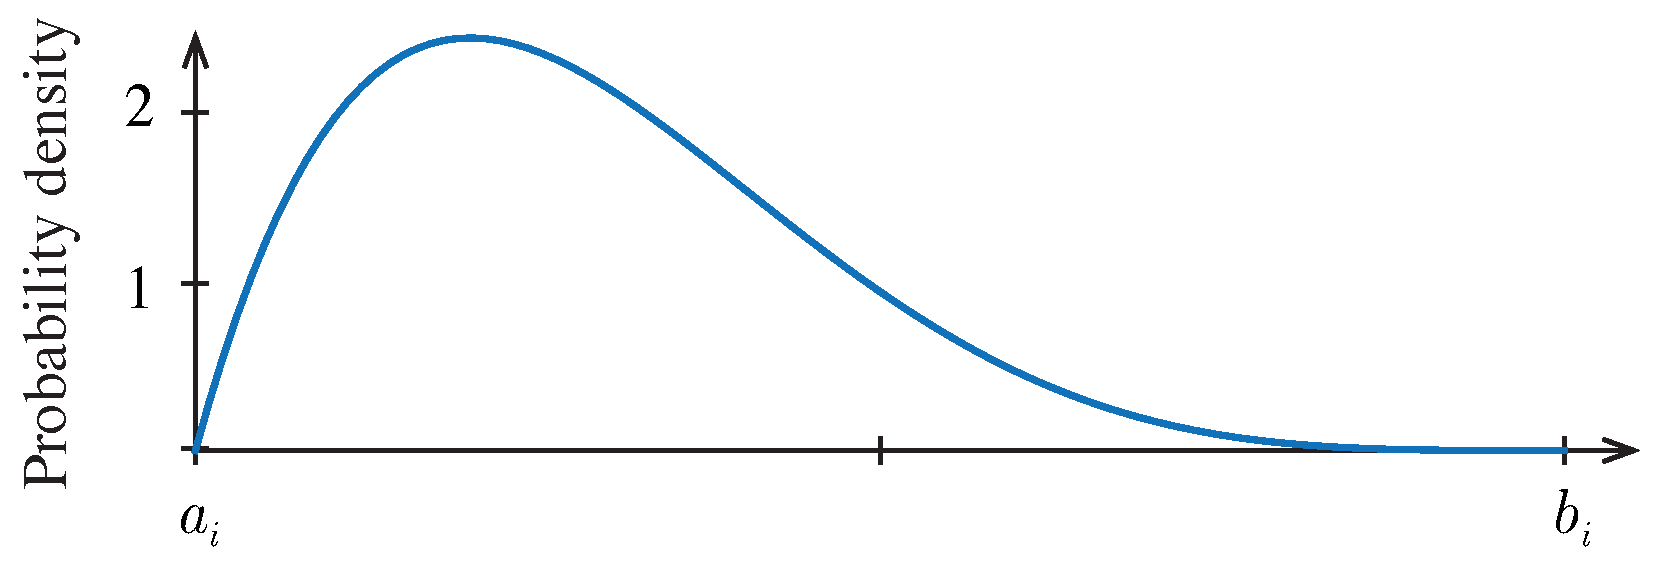
\includegraphics[width=1.0\columnwidth]{include/assets/figures/beta.pdf}
  \caption{The probability density of the beta distribution $\text{Beta}(2, 5, a_i, b_i)$.}
  \flab{beta}
\end{figure}

For illustration purposes, the uncertain parameters are assumed to be the
execution times of the tasks; in other words, $\vu = \vb$ and $\nu = \nt$.
Without loss of generality, the distribution of $\u_i$ or, equivalently, $\b_i$
is assumed to be a four-parametric beta distribution $\text{Beta}(\alpha_i,
\beta_i, a_i, b_i)$ where $\alpha_i$ and $\beta_i$ are the shape parameters, and
$a_i$ and $b_i$ are the endpoints of the support. The parameters $\alpha_i$ and
$\beta_i$ are set to 2 and 5, respectively, for all tasks. The left endpoint
$a_i$ is set to the best-case execution time of the task generated by the
\abbr{TGFF} tool, and the right endpoint $b_i$ is set to be 20\% larger than
$a_i$. The shape of such distributions is illustrated in \fref{beta}. The
correlations between the tasks of an application are generated based on the
structure of the corresponding directed acyclic graph produced by the
\abbr{TGFF} tool: the closer two tasks are in the graph, the stronger the
correlation between their execution times.

The construction of thermal \abbr{RC} circuits for the considered multiprocessor
platforms is delegated to the HotSpot tool \cite{skadron2004}; the output of the
tool is essentially a pair of a thermal capacitance matrix $\mC$ and a thermal
conductance $\mG$ matrix that appear in \eref{thermal-system}. The granularity
of power and temperature profiles, discussed in \sref{power-consumption} and
\sref{heat-dissipation}, is set to $10^{-5}$~s; in practice, this sampling rate
should be set to a value that is reasonable for the problem at hand.

Regarding interpolation, we rely on the open Newton--Cotes rule, as motivated in
\sref{collocation-nodes}. The \token{IsLimitReached} subroutine in
\aref{construct} terminates the algorithm when it reaches a certain
interpolation level. The decision taken in \token{IsAccurateEnough} is based on
\eref{absolute-error} and \eref{relative-error}.

Lastly, let us remind that our experimental setup is publicly available
\cite{sources}. The configuration aspects that have not been explicitly
mentioned here can be found online, and the results presented below can be
readily reproduced.

\subsection{Application Timing}
The quantity of interest $\g$ considered in this subsection is the end-to-end
delay given in \eref{end-to-end-delay}, which is a scalar.

\subsection{Power Consumption}
Let the quantity of interest $\g$ be the total energy given in
\eref{total-energy}, which is a scalar.

\subsection{Heat Dissipation}
In this subsection, the quantity of interest $\g$ is the temperature profile
$\mQ$ of the system calculated using \eref{thermal-system}. The profile is an
$\np \times \ns$ matrix, and, therefore, $\g$ is $\np \ns$-dimensional.


  \section{Conclusion} \slab{conclusion}
  In this paper, we have presented a framework for probabilistic analysis of
electronic systems. \updated{Given a description of the probability distribution
of the uncertain parameters present in the system under consideration and a
simulator of a metric of interest dependent on the parameters, the framework
prescribes the steps that need to be taken in order to computationally
efficiently obtain the probability distribution of the metric.}

The proposed approach is powered by hierarchical interpolation following a
hybrid adaptation strategy. The adaptivity makes the framework particularly
suited for problems with idiosyncratic behaviors and steep response surfaces,
which arise in electronic systems due to their digital nature.

The performance of our framework has been assessed by comparing it with the
performance of an advanced sampling technique. \updated{The experimental results
have shown that, for a fixed budget of evaluations of the metric, our approach
achieves higher accuracy compared to direct simulations.}

\updated{Finally, we would like to emphasize that, even though the framework has
been exemplified by considering a specific source of uncertainty and specific
metrics, it is general and can be successfully applied in many other settings.}


  \section*{Acknowledgments}
  The authors would like to thank Prof. Nicholas Zabaras and Dr. Xiang Ma from
Cornell University and Dr. Stefan Dirnstorfer from Munich Technical University
for the help with adaptive hierarchical interpolation and integration
techniques.


  \begingroup
    \bibliographystyle{IEEEtran}
    \bibliography{IEEEabrv,include/references}
  \endgroup
\end{document}
